\subsection{L’analisi del problema}

\subsubsection{Analisi delle funzionalità}
dai casi d'uso si deducono le funzionalità, che raggruppano i casi d'uso e sintetizzano le .. principali, con i relativi requisiti.

\begin{table}[htbp]
    \centering
    \begin{tabular} {|P{3.8cm}|P{4.5cm}|P{2.5cm}|P{4cm}|}
        \hline
        \textbf{Funzionalità} & \textbf{Tipo}                                                 & \textbf{Grado di complessità} & \textbf{Requisiti Collegati}                    \\
        \hline
        Login                 & Interazione esterno e lettura dati                            & semplice                      & R2F                                             \\
        \hline
        Registrazione         & Interazione esterno e memorizzazione dati                     & semplice                      & R1F                                             \\
        \hline
        EventiConfermati      & Interazione esterno e gestione dati                           & complessa                     & R3F, R8F                                        \\
        \hline
        EventiProposti        & Interazione esterno e gestione dati                           & complessa                     & R4F, R9F                                        \\
        \hline
        GestioneGruppi        & Interazione esterno e gestione dati                           & complessa                     & R15F, R16F                                      \\
        \hline
        GestioneProfili       & Interazione esterno e gestione dati                           & complessa                     & R17F, R18F, R19F                                \\
        \hline
        VisualizzaEvento      & Interazione esterno e gestione, lettura e memorizzazione dati & complessa                     & R5F, R6F, R7F, R8F, R9F, R10F, R11F, R12F, R14F \\
        \hline
        AggiornaEvento        & Gestione dati                                                 & complessa                     & R20F                                            \\
        \hline
        RecuperaImmagini      & Lettura dati                                                  & complessa                     & R13F                                            \\
        \hline
        ScritturaLog          & Memorizzazione dati                                           & semplice                      & R21F                                            \\
        \hline
    \end{tabular}

    \caption{Funzionalità}
    \label{<label>}
\end{table}

dopo l'analisi delle informazioni che ogni funzionalità deve gestire, si procede con l'analisi deli vincoli,
in cui si chiarificano i requisiti non funzionali, evidenziando le loro criticità e quali componenti ne vengono coinvolti.

\begin{table}[htbp]
    \centering
    \begin{tabular} {|P{3.5cm}|P{2cm}|P{3.5cm}|P{6cm}|}
        \hline
        \textbf{Requisito}                  & \textbf{Categorie} & \textbf{Impatto}                                                         & \textbf{Funzionalità}                                                                                                                       \\
        \hline
        Semplicità dell'interfaccia         & Usabilità          & Intuitività di utilizzo                                                  & Login, Registrazione, EventiConfermati, EventiProposti, GestioneGruppi, GestioneProfili, VisualizzaEvento, RecuperaImmagini                 \\
        \hline
        Velocità della ricerca dei dati     & Tempo di Risposta  & Maggiore reattività                                                      & EventiConfermati, EventiProposti, GestioneGruppi, GestioneProfili, RecuperaImmagini                                                         \\
        \hline
        Velocità di memorizzazione dei dati & Tempo di Risposta  & Maggiore reattività                                                      & Registrazione, AggiornaEvento, RecuperaImmagini                                                                                             \\
        \hline
        Controllo Accessi                   & Sicurezza          & Peggiorano tempo di risposta e usabilità, migliorano la privacy dei dati & EventiConfermati, EventiProposti, GestioneGruppi, GestioneProfili, VisualizzaEvento                                                         \\
        \hline
        Protezione dei\linebreak Dati       & Sicurezza          & Peggiorano tempo di risposta, migliorano la privacy dei dati             & Login, Registrazione, EventiConfermati, EventiProposti, GestioneGruppi, GestioneProfili, VisualizzaEvento, AggiornaEvento, RecuperaImmagini \\
        \hline
        Scalabilità delle richieste         & Tempo di Risposta  & Minor degradamento delle prestazioni                                     & EventiConfermati, EventiProposti, AggiornaEvento, RecuperaImmagini                                                                          \\
        \hline
    \end{tabular}
    \caption{Vincoli}
\end{table}


maschere, che rappresentano l'interfaccia utente.
\clearpage


\begin{table}[htbp]
    \centering
    \begin{tabular} {|P{7.3cm}|P{8cm}|}
        \hline
        \textbf{Funzionalità} & \textbf{Scomposizione}                                                                                                                            \\
        \hline
        EventiConfermati      & VisualizzaEvento                                                                                                                                  \\
        \hline
        EventiProposti        & VisualizzaEvento                                                                                                                                  \\
        \hline
        VisualizzaEvento      & CreaEvento, ModificaEvento, ConfermaEvento, DisdiciEvento, CondividiConLink, CondividiAiGruppi, CaricaImmagini, EliminaImmagini, ConfermaImmagini \\
        \hline
        GestioneGruppi        & CercaProfili, AggiungiProfiloAlGruppo, CreaGruppo                                                                                                 \\
        \hline
        CercaProfili          & AggiungiProfilo                                                                                                                                   \\
        \hline
        GestioneProfili       & CambiaProfilo                                                                                                                                     \\
        \hline
    \end{tabular}
    \caption{Scomposizione delle funzionalità}

\end{table}

\subsubsection{Architettura logica}

Il seguente diagramma delle classi rappresenta la parte di modello del dominio relativa al sistema. \\

\begin{figure}[h!]
    \begin{center}
        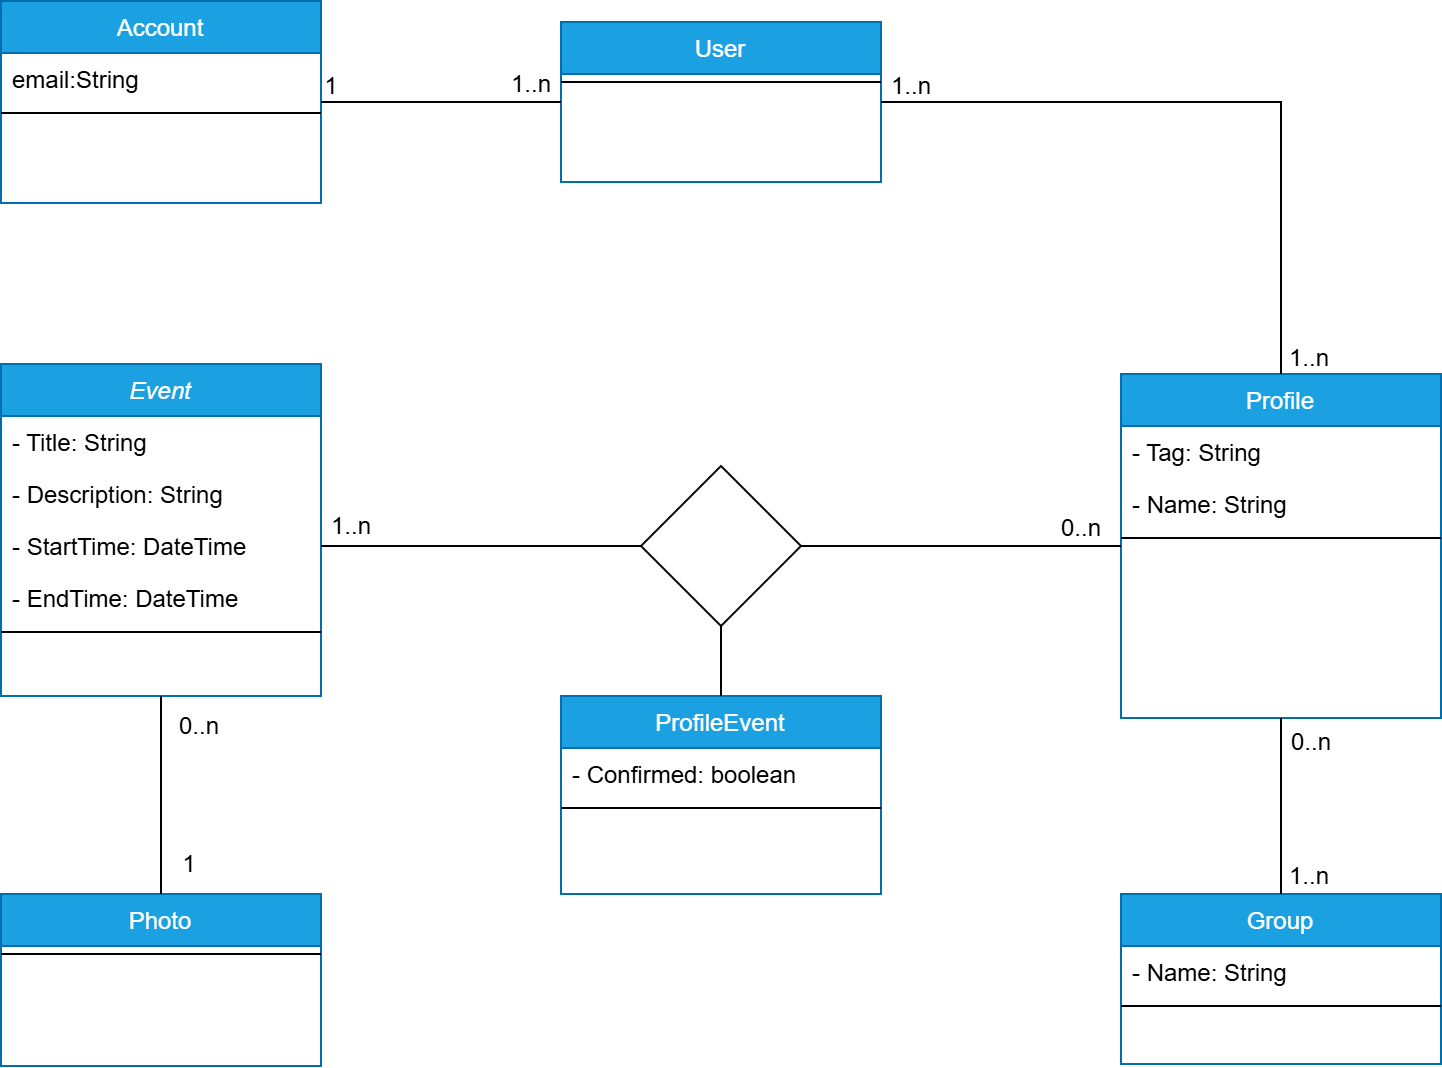
\includegraphics[width=\textwidth]{ModelloDominio.png}
        \caption{Modello del Dominio}
    \end{center}
\end{figure}

\begin{figure}[h!]
    \begin{center}
        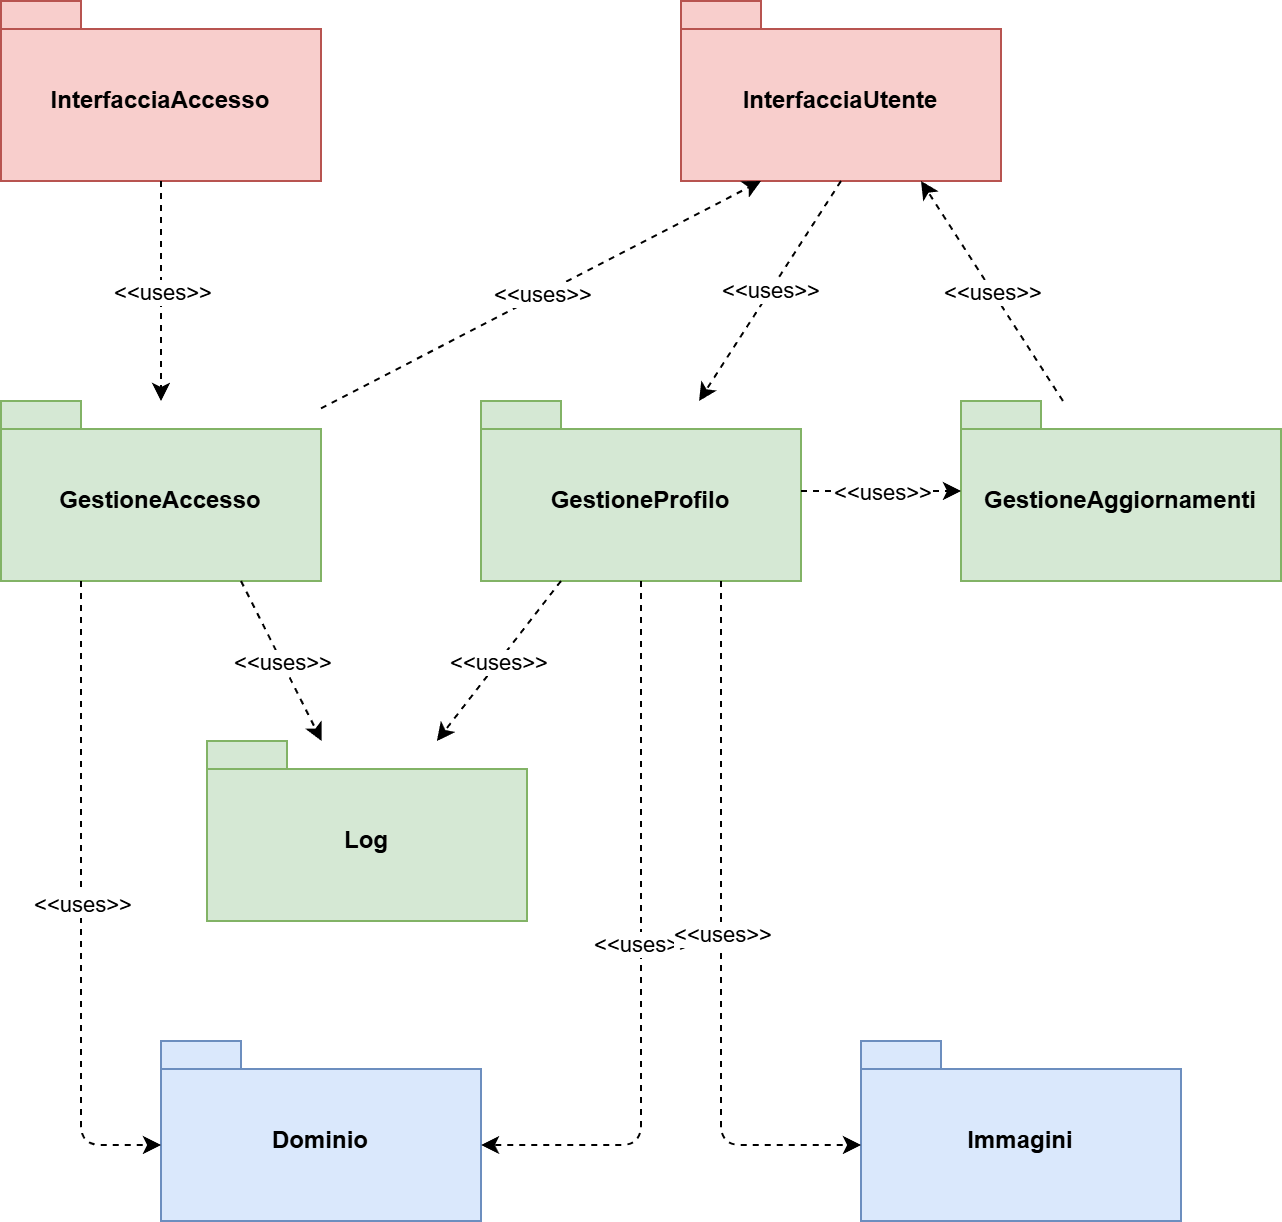
\includegraphics[width=\textwidth]{DiagrammaPackage.png}
        \caption{Diagramma dei Package}
    \end{center}
\end{figure}



\begin{figure}[h!]
    \begin{center}
        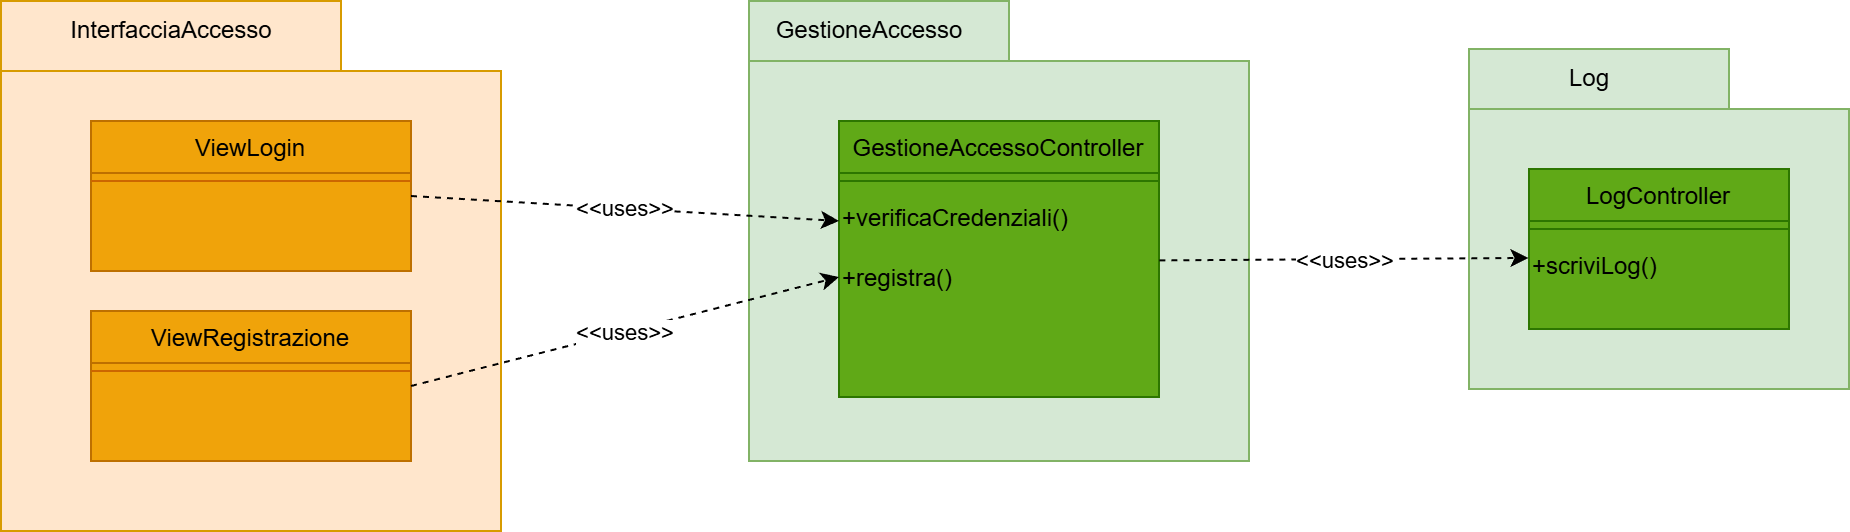
\includegraphics[width=\textwidth]{GestioneAccesso.png}
        \caption{Diagramma delle classi: interfacca e gestione accesso}
    \end{center}
\end{figure}


\begin{figure}[h!]
    \begin{center}
        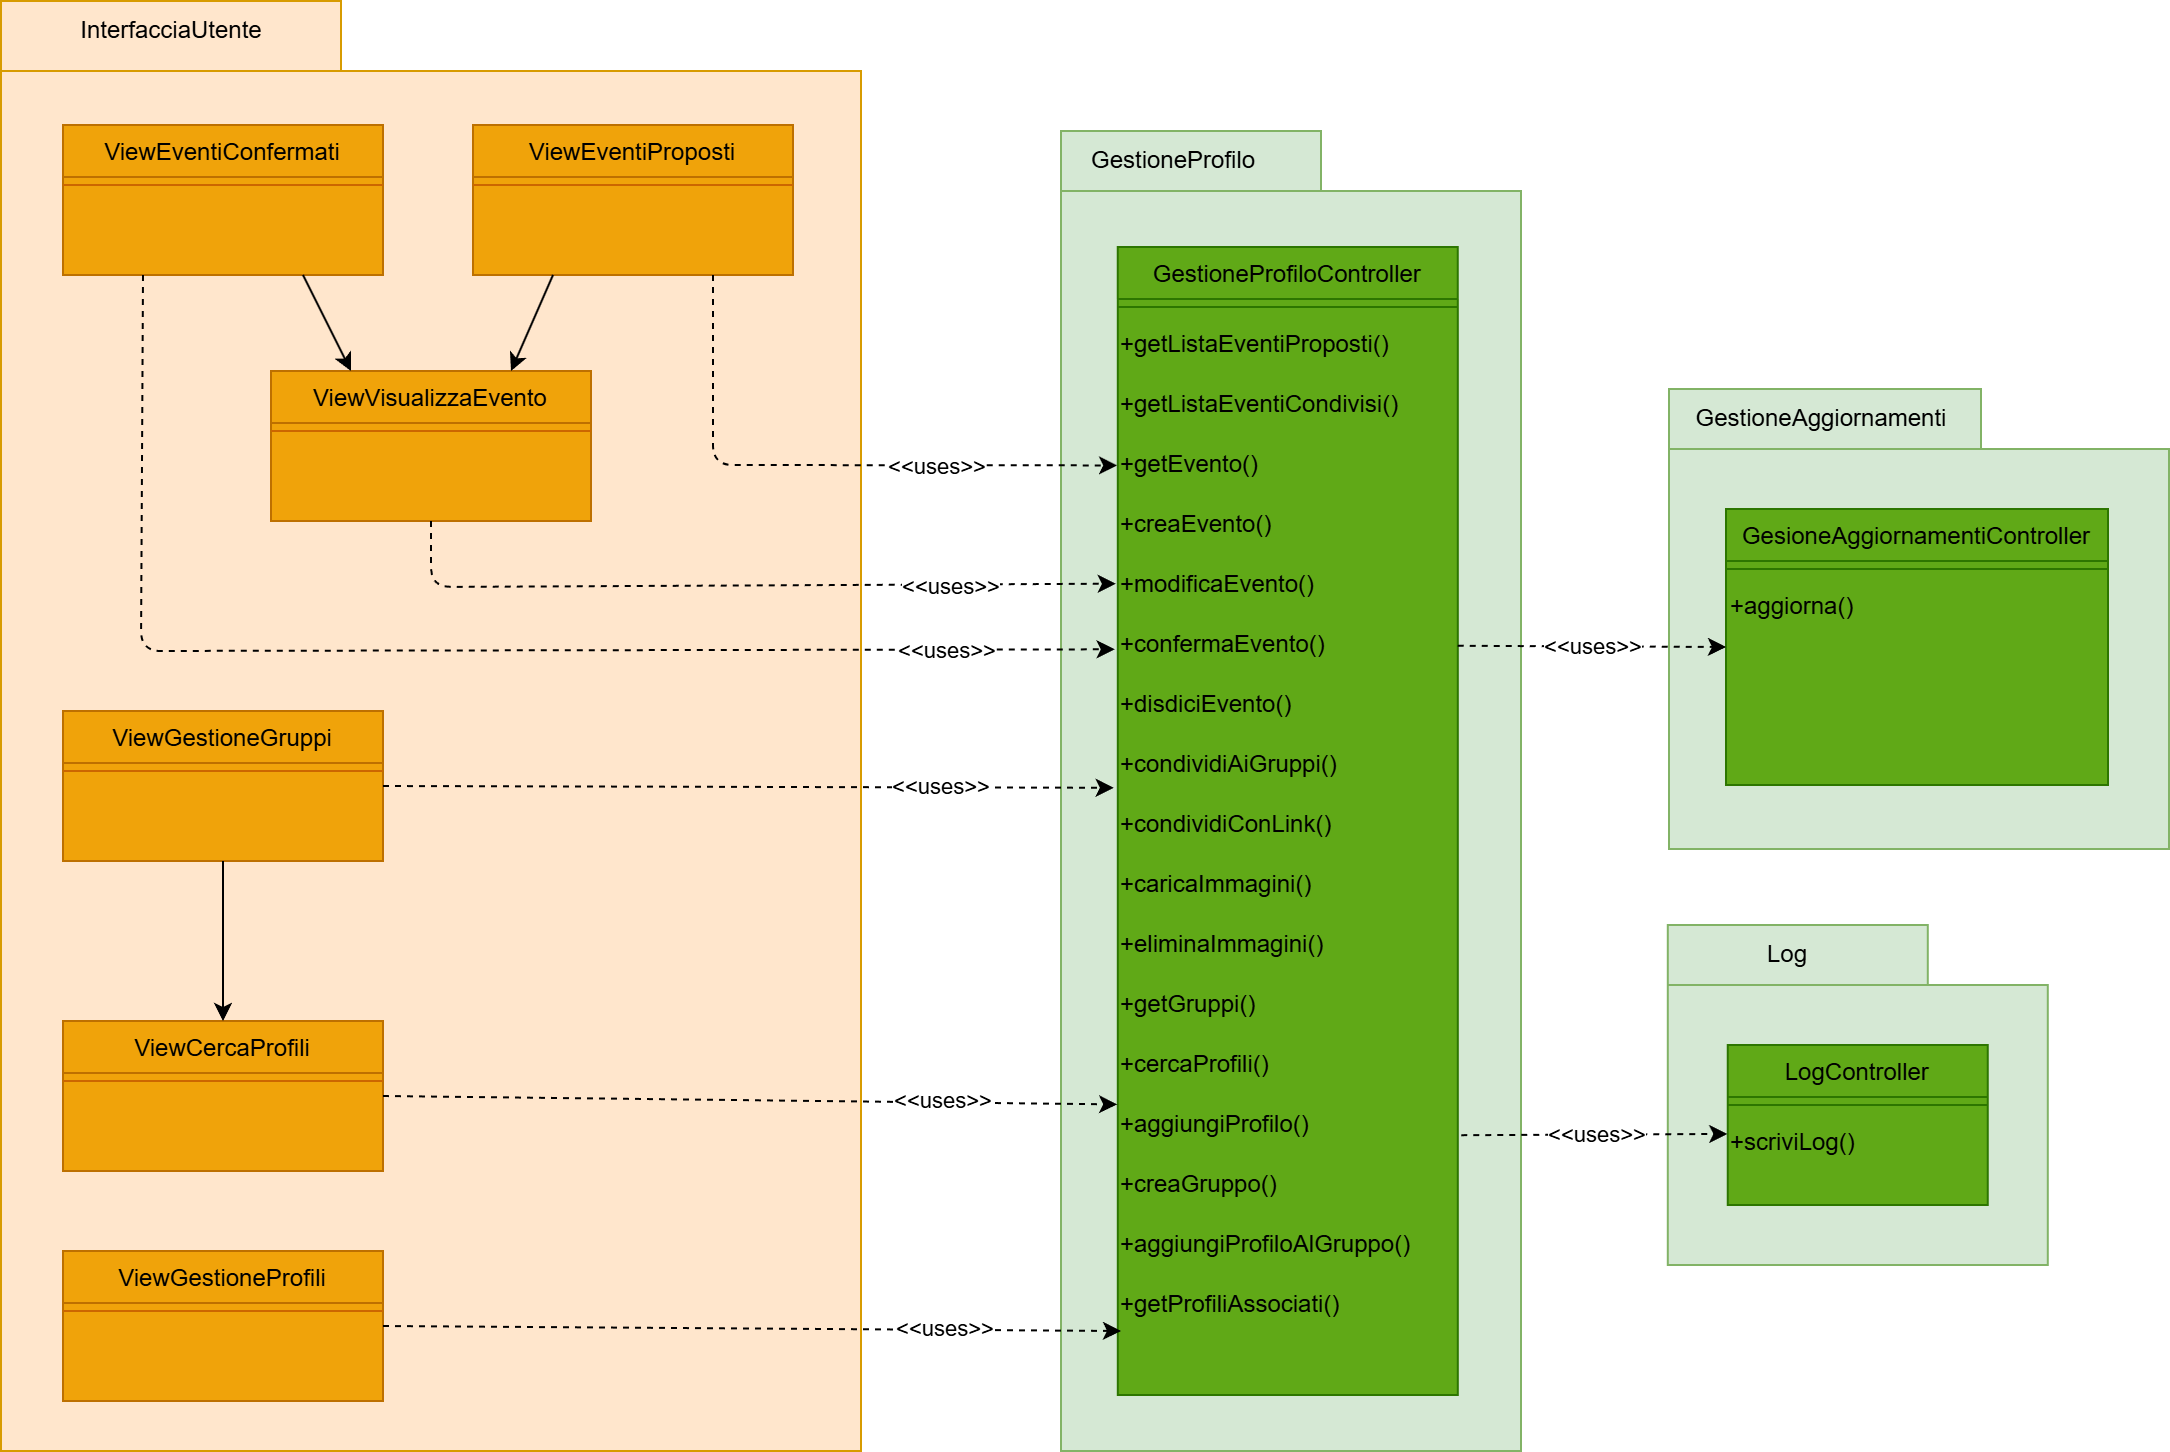
\includegraphics[width=\textwidth]{GestioneProfilo.png}
        \caption{Diagramma delle classi: interfacca utente, gestione profilo ed aggiornamenti}
    \end{center}
\end{figure}
\clearpage